В контексте автоматизации определение местоположения объекта обеспечивает более гибкое управление технологическим процессом (например, в составе SCADA-систем).

Существуют следующие применения радиометок:

\begin{itemize}
    \item отслеживание объектов на складах: пометив каждый объект <<радиометкой>>, организация получает возможность быстрого нахождения нужного предмета, экономно сокращая время и ресурсы машин; становится реальной возможность быстрого подсчёта продукции на складах без необходимости хранения данных в сложных базах данных;
    \item отслеживание движения механизмов и объектов на конвейерах: благодаря данной возможности, можно строить модели передвижения и работы всей текущей системы в целом, улучшать производительность и экономичность данной системы;
    \item отслеживание движения рабочего персонала (управление предприятием): позволяет исключить простой рабочего времени и с точностью определить график времени рабочего.
\end{itemize}

В целом, радиометки улучшают качество и безопасность автоматической системы управления.

В зависимости от конкретных целей использования радиометок, задача обеспечения необходимой точности будет различаться. Например, для определения текущего местоположения накопителя или грузовика во дворе, будет достаточной точность в пределах 2-3 метров. Однако, для определения точной ячейки на складе хранения валов диаметром 30 см, нужна будет сантиметровая точность. Вместе с точностью растут и требования к конечному устройсту, такие как \textbf{частота работы}. Помимо высокой частоты, устройство должно использовать свободный частотный диапазон: например, 433 МГц или 2.4 ГГц (Wi-Fi).

С развитием промышленной автоматизации, крупные компании заметили преимущества SCADA-систем и стали использовать их для сбора, анализа и отображения информации с датчиков, а также корректирования дальнейшего управления на основе этой информации. Используя <<радиометки>>, система может корректировать регулирование на основе пространственного положения объекта, что увеличивает гибкость и надёжность системы.

Архитектура применения радиометок в SCADA-системе представлена на рисунке~\ref{fig:scada}.

\begin{figure}[ht]
    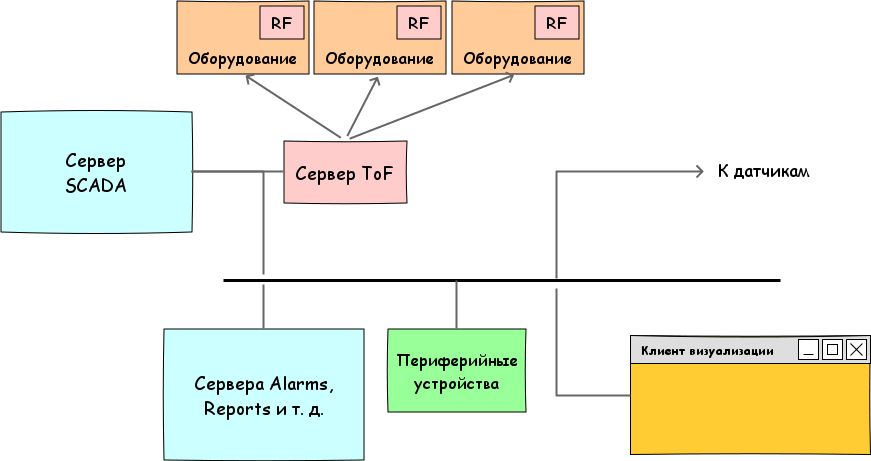
\includegraphics[width=1\linewidth]{Figures/scada.png}
    \caption{Применение радиометок в SCADA-системе}
    \label{fig:scada}
\end{figure}

Здесь RF - радиометка, отвечающая на полученное сообщение заданным сигналом (по запросу опрос-сервера).
